\graphicspath{{./design/}}

\chapter{Design}
% {{{
\label{cha:Design}

% {{{

A very modular approach to the design of the system was taken. A number of
required components was identified and categorised. The main component
categories of the system are:

\begin{itemize}
  \item Simulation I/O - handles input and output of data
  \item Coders - encodes and decodes symbols
  \item Compressors - drivers behind the compression
  \item Visualisation - displays the simulation data
  \item General components - general transformations
  \item Method specific components - components specific to a particular
  compression scheme
  \item Verification components - verify and record various aspects of the
  system
\end{itemize}

A brief overview of the different components and how they are used is provided
for in Section \ref{sec:design_overview}, while Section
\ref{sec:design_visualisation} will provide more detail into the
visualisation components of the system.

% }}}

\section{Overview}
% {{{
\label{sec:design_overview}

The executables of the system are within the Compressors and Visualisation
component categories, there are multiple executables so that
compression/decompression does not require a GUI being available.

The compression program (within Compressors or Visualisation), will use the
Simulation I/O components to read the molecular data, which will then be
transformed using the General components, the output of which will be used by
the Coders and Visualisation components. The Coders may have their own specific
components (Method specific components), which will be used to perform the
encoding/decoding of symbols. The Verification component will connect to the
various other components that it is measuring.

See figure TODO for a schematic diagram of all the components of the system,
and how they relate to each other.

% TODO: add diagram of components, and how they link up
[provide a schematic diagram of all the components and how they link up].

% }}}

\section{Visualisation}
% {{{
\label{sec:design_visualisation}

% {{{

With regards to the visualisation category, there are a number of components
within it, each of which will be discussed in this section.

\begin{itemize}
  \item Water point rendering (Section \ref{sub:design_waterpoint})
  \item Metaballs rendering (Section \ref{sub:design_metaballs})
  \item Water cluster visualisation (Section \ref{sub:design_watercluster})
  \item Quantisation error visualisation (Section \ref{sub:design_quanterror})
\end{itemize}

% }}}

\subsection{Water point rendering}
% {{{
\label{sub:design_waterpoint}

This rendering technique is the simplest of all the visualisation techniques in
the system. An almost transparent point will be drawn for each of the water
molecules. The points will be almost transparent so that a sense of the size of
the volume can be seen; as more water molecules overlap on the screen, the more
pronounced the colour at that point will be. See figure
\ref{fig:design_waterpoint}.

\begin{figure}[h!]
  \begin{center}
    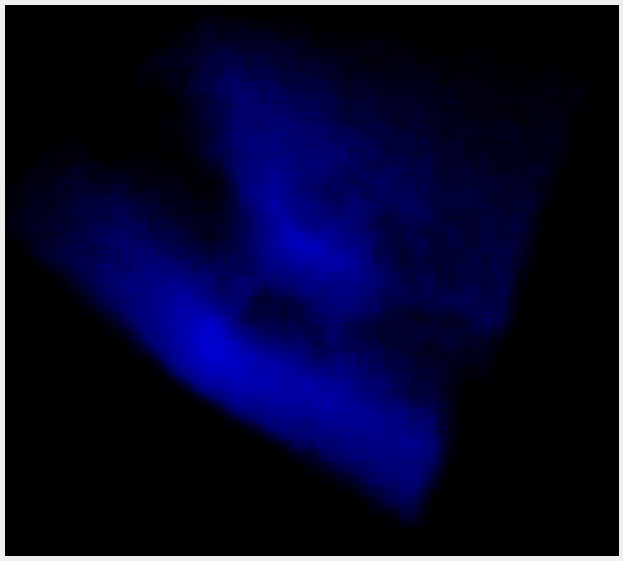
\includegraphics[width=70mm]{waterpoint}
  \end{center}
  \caption{Water point rendering, each point represents a water molecule}
  \label{fig:design_waterpoint}
\end{figure}

% }}}

\subsection{Metaballs rendering}
% {{{
\label{sub:design_metaballs}

The metaballs technique (Section \ref{sub:background_metaballs}) was chosen as
an alternative way to visualise the water volume in the molecular simulation as
it will group the water molecules together, hence providing some clutter
reduction. See figure TODO. The boundary of the water volume can be clearly
seen with metaballs, with water point rendering the boundary is not as clearly
visible.

% TODO: implement and compare marching tetrahedrons and marching cubes
[TODO: implement marching cubes, compare to marching tetrahedra, say which was
chosen as final implementation and why]

To determine the surface of the volume, the marching tetrahedrons algorithm was
used. Marching tetrahedrons was chosen over marching cubes for surface
extraction as it was easier to implement due to there is no ambiguity handling,
nor are lookup tables needed for the algorithm.

As the molecular data will need to be explored and displayed in real time, the
mesh obtained from the surface extraction will need to be simplified. This can
be accomplished by either increasing the grid size when sampling the volume to
determine the surface, or by mesh decimation. As mesh decimation provides more
control over what the final surface will look like, a mesh decimation algorithm
has been implemented.

Mesh decimation will be accomplished using the vertex clustering approach.
Vertex clustering was used instead of geometric decimation as it is more
computationally efficient and it integrates well with the surface extraction
part of the rendering process.

[TODO: implement another decimation approach to see what the speed differences
are?]

[TODO: insert final image]

% }}}

\subsection{Water cluster visualisation}
% {{{
\label{sub:design_watercluster}

Ribbon

[TODO: insert final image]

% }}}

\subsection{Quantisation error visualisation}
% {{{
\label{sub:design_quanterror}

[TODO: insert final image]

% }}}

% }}}

% }}}

% {{{

\newpage
\section{My questions (NOT TO BE INCLUDED IN FINAL REPORT)}

\begin{enumerate}

  \item
  I know that the tense of this chapter is quite confused. It has to do with
  the way that I was thinking when I typed this up (some of the stuff hasn't
  been implmented yet). I'm assuming that this chapter should phrase things in
  the past tense? i.e. the system \emph{was} designed with such and such in
  mind.

  \item
  I imagine that this chapter may change or be rephrased as the implementation
  progresses.

  \item
  How much detail should we go into for the design chapter? I couldn't find
  much to say without going into implementation details.

  \item
  As was mentioned, the design chapter shouldn't be a list and description of
  all the components, but all the components are very straight forward and
  relatively simple, especially for the visualisation...

  \item
  How much of this chapter will overlap with the implementation chapter?
  That is assuming that there will be an implementation chapter?

\end{enumerate}

% }}}
